\chapter{Desarrollo}

\section{Introducción}
En este capítulo, detallaremos el desarrollo de las mejoras implementadas en el planificador a corto plazo basado en Redes de Petri para el sistema operativo FreeBSD. El trabajo realizado se fundamenta en la colaboración y continuidad de proyectos previos desarrollados por estudiantes de nuestra institución.\par

La comprensión y depuración del código existente, así como la adaptación de los archivos del código fuente de FreeBSD relacionados con el planificador 4BSD, fueron tareas esenciales en nuestro proceso de desarrollo. Este esfuerzo intenta reflejar buenas prácticas en ingeniería de software, siendo ésta, una prioridad durante las primeras etapas de desarrollo. Nuestro enfoque integró principios de trabajo en equipo y metodologías ágiles, permitiendo una iteración continua y mejorada sobre el código. A lo largo del desarrollo, se implementaron prácticas de gestión de versiones y estrategias de ramificación para garantizar la calidad y estabilidad del código en cada una de sus etapas. En las siguientes secciones, se detallarán las metodologías utilizadas y los módulos específicos desarrollados, subrayando la importancia de cada componente en el contexto del planificador 4BSD.\par


\section{Metodologías de trabajo}
Para abordar el desarrollo de este proyecto de manera efectiva, establecimos una serie de metodologías de trabajo que nos permitieron mantener una organización rigurosa y una documentación detallada en cada etapa del proceso. Nuestro objetivo era no solo avanzar de manera sistemática, sino también crear un recurso valioso para futuros trabajos en este ámbito.\par

La primera etapa consistió en una profunda revisión del informe del trabajo integrador previo, así como del código base de los archivos de interés en el planificador 4BSD. Este proceso se realizó de forma iterativa, asegurándonos de comprender y extender la documentación de ambos componentes antes de proceder. Ampliar la documentación en esta etapa de análisis inicial, fue crucial para establecer una base sólida sobre la cual construir el resto del proyecto.\par

Una vez completada la fase de comprensión y documentación, planificamos nuestras metodologías de trabajo, enfocándonos en estrategias que facilitaran la colaboración y la gestión del proyecto. Implementamos una estrategia de ramas estandarizada en el repositorio fork de FreeBSD, permitiendo un control preciso de las versiones y facilitando la integración continua. Además, creamos un repositorio externo dedicado a almacenar toda la documentación y los recursos necesarios para el desarrollo, garantizando un acceso fácil y organizado a la información relevante.\par

Estas metodologías no solo nos permitieron trabajar de manera ordenada y eficiente, sino que también sentaron las bases para una colaboración efectiva y una fácil transición del conocimiento. En las siguientes secciones, se detallarán las estrategias específicas utilizadas.\par

\subsection{Estrategia de ramificación}
Definir una estrategia de ramificación o \textit{branch strategy} en los proyectos es fundamental para mantener el control sobre el flujo de trabajo, la organización del proyecto y asegurar que las modificaciones se integren sin problemas en la rama principal del código. Una estrategia bien definida establece un conjunto de reglas claras y consistentes para la creación y fusión de ramas de código.\par

Además, esta estrategia facilita el mantenimiento de un historial completo y bien organizado de las modificaciones realizadas al código, lo cual es esencial para el seguimiento y la continuidad del proyecto. En nuestro caso, definimos el prefijo de branches utilizando los apellidos de los integrantes del grupo de trabajo, como por ejemplo, \texttt{\textbf{DrudiGoldmanPI/}}. Este enfoque nos ayuda a identificar y localizar fácilmente todos los cambios realizados en este proyecto integrador.\par

Para definir los nombres de las ramas, establecimos tres casos principales por los cuales se crearían nuevas ramas:

\begin{itemize}
    \item \textbf{Testing}: Ramas creadas para realizar pruebas y verificar que ciertas partes del código fuente funcionen según lo esperado. Este tipo de ramas se utilizan principalmente para la depuración mediante el uso de logs.
    \item \textbf{Update}: Ramas dedicadas a la actualización del código base con las versiones más recientes de FreeBSD. Esto es especialmente relevante en la fase inicial del proyecto, cuando se deben integrar los cambios previos realizados en el proyecto integrador anterior.
    \item \textbf{Feature}: Ramas utilizadas para el desarrollo de nuevas funcionalidades o la adición de código no existente previamente. Estas ramas permiten la implementación y prueba de nuevas características sin afectar la estabilidad de la rama principal.
\end{itemize}

Con estos tres casos principales (o causas), se definió la estrategia de nombrado de ramas de la siguiente forma:

\begin{center}
    \texttt{\textbf{DrudiGoldmanPI/<CAUSA>\_<DESCRIPCIÓN>-<VERSION\_FREEBSD>}}
\end{center}

Donde \texttt{\textbf{<DESCRIPCIÓN>}} es una breve explicación del contenido de los cambios y \texttt{\textbf{<VERSION\_FREEBSD>}}, es la versión de FreeBSD que se utilizó para realizar los cambios.

Por ejemplo, \textit{DrudiGoldmanPI/feature\_cpuMonopolized-13.1.0} es una rama destinada a la implementación del módulo de monopolización, el cual se detalla más adelante en esta sección de desarrollo; mientras que \textit{DrudiGoldmanPI/update\_petriNetScheduler-12.3.0} corresponde a una rama utilizada para la actualización del planificador 4BSD, modelado mediante Redes de Petri, a la versión 12.3.0 del sistema operativo.\par

\subsection{Conventional Commits}
En nuestro proyecto, utilizamos la convención de \textit{Conventional Commits} para mantener un historial de cambios claro y consistente. Esta práctica facilita la lectura y comprensión de los cambios realizados, tanto para el equipo de desarrollo como para futuros colaboradores.\par

Los mensajes de \textit{commit} siguen un formato estandarizado que describe de manera concisa el tipo de cambio, la versión del sistema operativo afectada y una breve descripción de la modificación. A continuación, se presentan algunos ejemplos extraídos de nuestro proyecto:

\begin{itemize}
    \item \texttt{feat(13.1.0): Move thread lock before resource\_expulse\_thread()}
    \item \texttt{fix(13.1.0): Fix sched\_pickcpu for cases when resource\_choose\_cpu returns -1 (NOCPU)}
    \item \texttt{refactor(13.1.0): Change \textit{kernel} config file identifier}
    \item \texttt{feat(12.3.0): Short term scheduler modeling with PN - Add PI code to release/12.3.0}
\end{itemize}

Los tipos de cambios más comunes que utilizamos incluyen:
\begin{itemize}
    \item \textbf{feat}: Para la adición de nuevas funcionalidades.
    \item \textbf{fix}: Para la corrección de errores.
    \item \textbf{refactor}: Para modificaciones que mejoran el código sin alterar su funcionalidad.
\end{itemize}

Para la integración de cambios, hemos adoptado la estrategia de \textit{squash merge}. Esta técnica permite consolidar todos los cambios de una rama en un único \textit{commit} bien detallado, lo cual simplifica el historial del proyecto y facilita el seguimiento de avances importantes. Cada \textit{squash merge} incluye un resumen comprensivo de todos los \textit{sub-commits} que forman parte del cambio, garantizando así una documentación clara y precisa del progreso del proyecto.\par

\subsection{Repositorio de Documentación del Proyecto} \label{sect:wiki}

El repositorio de la documentación del proyecto está organizado de manera estructurada y detallada, facilitando el acceso y la gestión de la información relevante para el desarrollo del mismo. A continuación, se presenta una descripción breve de su estructura principal:

\begin{itemize}
    \item \textbf{Archivos del Proyecto}
          \begin{itemize}
              \item \textbf{Archivos de Migraciones:} Contiene subdirectorios correspondientes a diferentes versiones de migración del sistema, incluyendo archivos de configuración y código fuente relevante.
              \item \textbf{Logs:} Registro de eventos y mensajes generados durante pruebas y actualizaciones del sistema.
              \item \textbf{Módulos:} Módulos de \textit{kernel} adicionales para poner en funcionamiento los nuevos desarrollos.
              \item \textbf{Otros:} Programas auxiliares para seguir el comportamiento de las transiciones de la Red de Petri.
              \item \textbf{Programas de Test:} Programas utilizados para pruebas de rendimiento y funcionalidad.
          \end{itemize}
    \item \textbf{Documentación del Proyecto}
          \begin{itemize}
              \item \textbf{Uso del Repositorio:} Guías sobre cómo manejar las ramas y versiones del repositorio.
              \item \textbf{Iteraciones:} Detalles de las distintas iteraciones del proyecto.
          \end{itemize}
\end{itemize}

Esta organización meticulosa asegura que todos los aspectos del proyecto, desde el código fuente hasta la documentación y los informes, estén bien gestionados y accesibles para los miembros del equipo.\par

Para más detalles, puede acceder al repositorio de documentación del proyecto en: \url{https://github.com/drudilea/free-bsd-scheduler}.\par

\section{Módulo de actualizaciones}

El desarrollo del proyecto se organizó en módulos, cada uno con objetivos específicos y alcanzables para asegurar avances concretos en cada etapa.\par

En la fase inicial, nos enfocamos en una tarea esencial en cualquier proyecto de software: mantener la compatibilidad con las diferentes versiones del sistema operativo. De esta forma, obtuvimos beneficios significativos en términos de estabilidad y compatibilidad, resultando en un sistema más confiable. Además, estando alineados con la ultima versión del mismo, nos acerca a la posibilidad de contribuir al proyecto de una manera directa.\par

El trabajo comenzó con la versión 11 de FreeBSD, basado en el trabajo integrador previo realizado por Nicolás Papp y Tomás Turina, y se extendió hasta la última versión estable, la 13.1.\par

Para gestionar las actualizaciones de manera ordenada y efectiva, así como también, comprender mejor los cambios entre versiones; el módulo se dividió en tres etapas progresivas: actualización a la última \textit{release} de la versión 11, y actualizaciones a las versiones 12 y 13 de FreeBSD.\par


\subsection{Actualización al último \textit{release} de la versión 11}

En esta primera iteración se buscó llevar los cambios del proyecto integrador previo realizados en la versión 11.0.0 del sistema operativo FreeBSD a la última release de ésta versión, es decir, al 11.4.0.\par

Durante dicha actualización, nos encontramos con un cambio significativo que tuvo un impacto relevante en nuestro proyecto: la modificación en la función \verb|maybe_preempt()|. En la versión anterior, esta función se encargaba de determinar si un nuevo hilo debía tomar el control del procesador inmediatamente, reemplazando al hilo actual en ejecución. En caso afirmativo, se realizaba el cambio de contexto y comenzaba su ejecución, sustituyendo al hilo que se encontraba en el procesador.\par

En la versión más reciente, se introdujo una nueva estrategia, posponer el cambio de contexto para un momento más adecuado mediante un sistema de banderas. En lugar de realizar el cambio de contexto de manera inmediata, se implementó un mecanismo donde el hilo recién encolado establece el valor de la bandera \verb|td_owepreempt| en 1, indicando la necesidad de desalojar al que se encuentra en ejecución, para así tomar el control.\par

Si bien el metodo de preemption no se encuentra modelado en nuestra Red de Petri de Recursos, este cambio impactó en el código del planificador de nuestro trabajo ya que implicó la remoción de algunos disparos de transiciones que se provocaban en el cambio de contexto inmediato. Con la nueva estrategia, fue necesario ajustar el código de nuestra Red de Petri para reflejar el cambio en la política de planificación.\par

\subsection{Actualización a la versión 12}

Al comparar las diferencias entre las versiones 11.4.0 y 12.3.0 (último \textit{release}) de FreeBSD, no se encontraron cambios significativos en los archivos relevantes para nuestro proyecto del planificador. Debido a esto, no fue necesario realizar ajustes específicos para esta versión.\par


\subsection{Actualización a la versión 13}

La versión 13 trajo con ella varios cambios significativos en el código del planificador. Los cambios principales, y que mayor tiempo de análisis e investigación tomaron, fueron los cambios dentro de la función \verb|sched_switch()|, función encargada de realizar el cambio de contexto entre hilos en el planificador 4BSD.\par

El primero de ellos (ver Apéndice \ref{appendix:apA1}) ya se encuentra en la firma de la función y sus variables: previamente, \verb|newtd| era un parámetro de \verb|sched_switch()| que se utilizaba para indicar explícitamente el hilo que se iba a ejecutar a continuación. Sin embargo, en la versión 13, el parámetro \verb|newtd| se eliminó y con ello se simplificó la lógica de selección del hilo (ver Apéndice \ref{appendix:apA3}), teniendo que ajustar algunos disparos en la Red de Petri que previamente eran necesarios para mantener la coherencia de los recursos relacionados, con estos desencolados en el planificador.\par

En la versión 13 de FreeBSD, se realizó una reorganización significativa de los locks en la función \verb|sched_switch()| (ver Apéndice \ref{appendix:apA2}). Estos cambios introdujeron comportamientos inesperados en la red, como el disparo de transiciones no sensibilizadas que desajustaban el estado de la red y causaban fallos en el sistema. Después de depurar el código, identificamos que el problema principal era el manejo incorrecto de la transición \verb|RETURN_VOL|. Específicamente, el método \verb|resource_expulse_thread()| estaba disparando esta transición sin bloquear previamente el \verb|td_lock|. Sin este bloqueo, no era posible cambiar el estado del hilo, lo que impedía que regresara al estado de \verb|CAN_RUN| o listo para ejecutarse. Como resultado, ningún hilo podía ser ejecutado por los procesadores más de una vez, lo que bloqueaba el sistema. Tras realizar los ajustes necesarios, logramos resolver este problema y garantizar el correcto funcionamiento de la red.\par

\subsection{Resultados}

Durante la actualización a las diferentes versiones del sistema operativo FreeBSD, se logró garantizar el funcionamiento correcto de todas las versiones, lo cual fue un logro significativo. Esto permitió no solo mantener el proyecto al día, sino también adentrarnos en el código del sistema operativo y comprender su funcionamiento de manera más integral.\par

Se tuvo la oportunidad de leer y analizar el código fuente en profundidad. Esto nos permitió adquirir un conocimiento detallado del proyecto y nos familiarizó con su estructura y características particulares. Esta inmersión en el código nos brindó una base sólida para abordar tareas posteriores de manera más eficiente y efectiva.\par

Adicionalmente, durante el proceso de actualizaciones, se identificaron, realizaron y documentaron algunas mejoras respecto a versiones anteriores del proyecto. Dichas mejoras fueron registradas en el repositorio de documentación (apartado \ref{sect:wiki}); y algunas de ellas, en el presente documento, con el objetivo de mantener un registro detallado y accesible para trabajos futuros.\par

\subsection{Próximos pasos}

Como se desarrolló previamente, sostenemos la importancia de mantener el proyecto actualizado con las últimas versiones del sistema operativo FreeBSD para asegurar su eficiencia, seguridad y compatibilidad con tecnologías mas recientes.\par

Para lograr este objetivo, es esencial monitorear continuamente las actualizaciones y aplicar los cambios necesarios de manera oportuna. Esto evitará el rezago respecto a \textit{releases} más recientes y garantizará que el proyecto se beneficie de las últimas mejoras y correcciones de errores.\par

Mantener el software actualizado en proyectos de código abierto como FreeBSD no solo mejora el rendimiento y la seguridad, sino que también facilita una integración más estrecha con la comunidad de desarrolladores y usuarios. Estar al día con las actualizaciones permite recibir retroalimentación valiosa, contribuyendo al desarrollo colaborativo.\par

Para futuros trabajos en este proyecto, se recomienda priorizar la importancia de este aspecto y comprometerse a dedicar los recursos y el tiempo necesarios para llevar a cabo las actualizaciones de manera regular.\par

\section{Módulo de encendido/apagado de los procesadores}

Tras completar las actualizaciones del sistema operativo, el siguiente paso fue desarrollar una nueva funcionalidad enfocada en el control de los núcleos del procesador. Esta funcionalidad está diseñada para proporcionar una herramienta flexible que permita la gestión dinámica del encendido y apagado de los núcleos del procesador, con la expectativa de que futuros proyectos utilicen este módulo para optimizar el ahorro energético.\par

Este módulo es especialmente útil en escenarios donde la carga de trabajo varía significativamente, permitiendo controlar los núcleos durante periodos de baja demanda y ajustarlos cuando la carga aumenta. Aunque aún no se ha implementado una estrategia de ahorro energético, esta herramienta abre la puerta a desarrollos futuros que podrían aprovechar esta capacidad para reducir el consumo de energía y mejorar la eficiencia del sistema.\par

\subsection{Objetivos}

El objetivo general de esta sección, fue el desarrollo de una nueva funcionalidad dentro del \textit{scheduler} del sistema operativo FreeBSD que permita habilitar o deshabilitar los diferentes núcleos del procesador de manera dinámica.\par

Este objetivo principal se traduce en múltiples aplicaciones que pueden proporcionar ventajas significativas, tales como la optimización del uso de recursos de hardware bajo cargas de trabajo reducidas, la restricción de núcleos disponibles para aplicaciones específicas, y la capacidad de ajustar el estado de los procesadores en tiempo de ejecución.\par

\subsection{Primera Iteración: Implementación del Módulo de Encendido/Apagado mediante cambios en la Red de Petri}

Para iniciar la implementación del módulo de encendido/apagado de núcleos del procesador, se debatieron dos enfoques relacionados con la Red de Petri del sistema operativo. El primer enfoque proponía utilizar las plazas y transiciones ya existentes, estableciendo diferentes políticas a través de cambios en el código del \textit{scheduler}. El segundo enfoque, que fue el adoptado finalmente, implicaba la incorporación de nuevas plazas y transiciones en la Red de Petri para representar explícitamente el estado de los núcleos del procesador. Optamos por esta segunda opción porque nos permitió integrar el módulo de manera más fluida al sistema ya existente, sin hacer cambios drásticos en el núcleo del sistema operativo, y ampliando al mismo tiempo las capacidades de la Red de Petri. La principal ventaja de esta implementación, y motivador principal, fue que desde cualquier parte del sistema, simplemente disparando una transición, fuera posible activar o desactivar cualquier núcleo del procesador según sea necesario.\par

Con esta decisión en mente, el primer paso fue crear un indicador que permitiera conocer si cada procesador está encendido o apagado. Para esto, se añadió una nueva plaza en la Red de Petri, llamada \verb|PLACE_SUSPENDED|. La presencia o ausencia de un \textit{token} en esta plaza indica si un procesador está disponible para encolar y ejecutar hilos.\par

La plaza \verb|PLACE_SUSPENDED| está acompañada de dos transiciones que manejan el \textit{token} correspondiente: \verb|TRAN_SUSPEND_PROC| para deshabilitar el núcleo, y \verb|TRAN_WAKEUP_PROC| para habilitarlo nuevamente. Se añadió un arco inhibidor a la transición que libera el recurso para asegurar que la plaza funcione como un recurso único. Una vez que un procesador está deshabilitado, solo la transición que lo habilita de nuevo queda sensibilizada.\par

En resumen, la plaza \verb|PLACE_SUSPENDED| controla las transiciones de encolado, tanto de la cola específica de la CPU, como de la cola global. Cuando la CPU está suspendida, impide que nuevos hilos se añadan a su cola y se ejecuten. Sin embargo, es importante destacar que este desarrollo no elimina los hilos que ya estaban en la cola de la CPU antes de que se deshabilitara. Es decir, los hilos ya encolados seguirán siendo ejecutados, pero no podrán volver a la cola de la CPU inhabilitada. Esta lógica está reflejada en la Red de Petri, donde la nueva plaza de suspensión solo afecta a las transiciones de encolado y desencolado, sin interferir en la ejecución de hilos ni en la transición específica de desencolado del procesador (\verb|TRAN_UNQUEUE|).\par

\begin{figure}[H]
    \centering
    \vspace*{0.1in}
    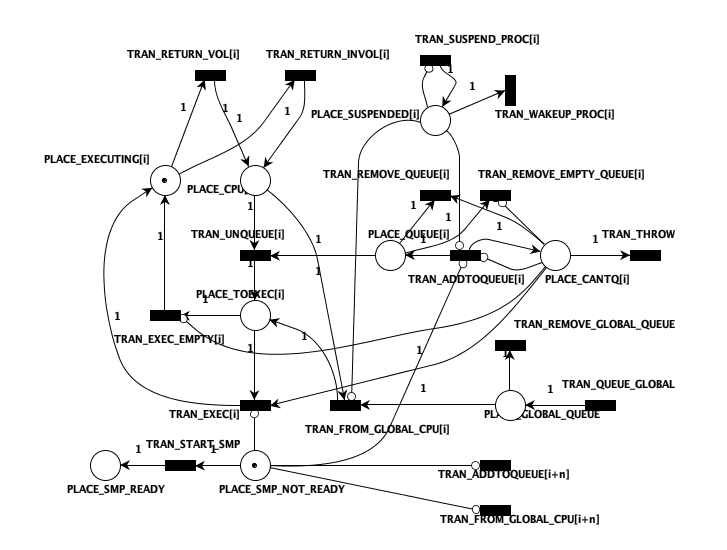
\includegraphics[width=0.8\textwidth]{./images/cpuOnOff-1st-iteration.png}
    \caption{Primera iteración del módulo de encendido/apagado de núcleos del procesador.}
    \label{fig:cpu-on-off-1st-iteration}
\end{figure}

Como primer paso para implementar esta funcionalidad a nivel de código, nos centramos en ajustar las matrices fundamentales que soportan el funcionamiento de la Red de Petri: la matriz base y la matriz de incidencia. Estas matrices son cruciales para la representación y el manejo de las transiciones y plazas en la Red de Petri.\par

La matriz base, que define la estructura inicial de la Red de Petri, necesitaba ser actualizada para reflejar las nuevas plazas y transiciones introducidas. Específicamente, agregamos entradas para la nueva plaza \verb|PLACE_SUSPENDED| y las transiciones asociadas (\verb|TRAN_SUSPEND_PROC| y \verb|TRAN_WAKEUP_PROC|). Esta modificación asegura que la estructura de la red pueda manejar los cambios en el estado de los núcleos del procesador, permitiendo que el sistema registre y gestione correctamente los \textit{tokens} en la plaza de suspensión.\par

\renewcommand{\arraystretch}{1.5}
\setlength{\tabcolsep}{10pt}

\begin{table}[H]
    \centering
    \begin{tabular}{|c|c|c|c|c|c|c|c|c|}
        \hline
        1 & 0  & -1 & 0  & 0  & 0  & 0  & -1 & 0  \\
        \hline
        1 & -1 & 0  & 0  & 0  & 0  & 0  & -1 & -1 \\
        \hline
        0 & -1 & 0  & 0  & 1  & 1  & -1 & 0  & 0  \\
        \hline
        0 & 1  & -1 & -1 & 0  & 0  & 1  & 0  & 0  \\
        \hline
        0 & 0  & 1  & 1  & -1 & -1 & 0  & 0  & 0  \\
        \hline
    \end{tabular}
    \caption{Matriz base inicial.}
    \label{tabla:matriz_base_pre}
\end{table}

\begin{table}[H]
    \centering
    \begin{tabular}{|c|c|c|c|c|c|c|c|c|c|c|}
        \hline
        1                      & 0                      & -1                     & 0                      & 0                      & 0                      & 0                      & -1                     & 0                      & \cellcolor{lightgray}0 & \cellcolor{lightgray}0  \\
        \hline
        1                      & -1                     & 0                      & 0                      & 0                      & 0                      & 0                      & -1                     & -1                     & \cellcolor{lightgray}0 & \cellcolor{lightgray}0  \\
        \hline
        0                      & -1                     & 0                      & 0                      & 1                      & 1                      & -1                     & 0                      & 0                      & \cellcolor{lightgray}0 & \cellcolor{lightgray}0  \\
        \hline
        0                      & 1                      & -1                     & -1                     & 0                      & 0                      & 1                      & 0                      & 0                      & \cellcolor{lightgray}0 & \cellcolor{lightgray}0  \\
        \hline
        0                      & 0                      & 1                      & 1                      & -1                     & -1                     & 0                      & 0                      & 0                      & \cellcolor{lightgray}0 & \cellcolor{lightgray}0  \\
        \hline
        \cellcolor{lightgray}0 & \cellcolor{lightgray}0 & \cellcolor{lightgray}0 & \cellcolor{lightgray}0 & \cellcolor{lightgray}0 & \cellcolor{lightgray}0 & \cellcolor{lightgray}0 & \cellcolor{lightgray}0 & \cellcolor{lightgray}0 & \cellcolor{lightgray}1 & \cellcolor{lightgray}-1 \\
        \hline
    \end{tabular}
    \caption{Matriz base: Primera iteración del módulo de encendido/apagado.}
    \label{tabla:matriz_base_post}
\end{table}

Por otro lado, la matriz de incidencia describe cómo las transiciones afectan a las plazas y viceversa. Actualizar esta matriz implicó modificar las relaciones entre las nuevas transiciones y las plazas afectadas. Concretamente, tuvimos que ajustar las entradas para reflejar el impacto de las transiciones de habilitación y deshabilitación de los núcleos en las plazas correspondientes. Esto incluye la configuración de los arcos inhibidores que garantizan que los cambios en el estado del procesador se gestionen correctamente.\par

\renewcommand{\arraystretch}{1.5}
\setlength{\tabcolsep}{10pt}

\begin{table}[H]
    \centering
    \begin{tabular}{|c|c|c|c|c|c|c|c|c|}
        \hline
        1 & 0 & 0 & 1 & 0 & 0 & 0 & 0 & 1 \\
        \hline
        0 & 0 & 0 & 0 & 0 & 0 & 0 & 0 & 0 \\
        \hline
        0 & 0 & 0 & 0 & 0 & 0 & 0 & 0 & 0 \\
        \hline
        0 & 0 & 0 & 0 & 0 & 0 & 0 & 0 & 0 \\
        \hline
        0 & 0 & 0 & 0 & 0 & 0 & 0 & 0 & 0 \\
        \hline
    \end{tabular}
    \caption{Matriz de incidencia inicial.}
    \label{tabla:matriz_incidencia_pre}
\end{table}

\begin{table}[H]
    \centering
    \begin{tabular}{|c|c|c|c|c|c|c|c|c|c|c|}
        \hline
        1                      & 0                      & 0                      & 1                      & 0                      & 0                      & 0                      & 0                      & 1                      & \cellcolor{lightgray}0 & \cellcolor{lightgray}0 \\
        \hline
        0                      & 0                      & 0                      & 0                      & 0                      & 0                      & 0                      & 0                      & 0                      & \cellcolor{lightgray}0 & \cellcolor{lightgray}0 \\
        \hline
        0                      & 0                      & 0                      & 0                      & 0                      & 0                      & 0                      & 0                      & 0                      & \cellcolor{lightgray}0 & \cellcolor{lightgray}0 \\
        \hline
        0                      & 0                      & 0                      & 0                      & 0                      & 0                      & 0                      & 0                      & 0                      & \cellcolor{lightgray}0 & \cellcolor{lightgray}0 \\
        \hline
        0                      & 0                      & 0                      & 0                      & 0                      & 0                      & 0                      & 0                      & 0                      & \cellcolor{lightgray}0 & \cellcolor{lightgray}0 \\
        \hline
        \cellcolor{lightgray}1 & \cellcolor{lightgray}0 & \cellcolor{lightgray}0 & \cellcolor{lightgray}0 & \cellcolor{lightgray}0 & \cellcolor{lightgray}0 & \cellcolor{lightgray}1 & \cellcolor{lightgray}0 & \cellcolor{lightgray}0 & \cellcolor{lightgray}1 & \cellcolor{lightgray}0 \\
        \hline
    \end{tabular}
    \caption{Matriz de incidencia: Primera iteración del módulo de encendido/apagado.}
    \label{tabla:matriz_incidencia_post}
\end{table}

Como parte de los ajustes realizados en las matrices, se incorporó una nueva función, \linebreak\verb|toggle_active_cpu()|, al archivo de métodos auxiliares de la Red de Petri. Esta función puede ser invocada desde un módulo del \textit{kernel} y está diseñada para alternar el estado de un CPU especificado como parámetro. La función verifica si la transición asociada está sensibilizada y, si es así, procede a dispararla. En resumen, esta adición permite seleccionar y alternar el estado de un procesador, que puede ser suspendido o activado según sea necesario, y se gestiona de manera externa al flujo principal del kernel, permitiendo así un control en ejecución del estado de habilitación de la CPU.\par

Tras la implementación de esta funcionalidad, nos encontramos con un problema inesperado: la funcionalidad no se comportaba como se había previsto. Específicamente, recibimos alertas indicando que algunas transiciones no estaban sensibilizadas durante los intentos de disparo. El proceso de depuración reveló que el problema estaba relacionado con el comportamiento del \textit{scheduler} cuando no había hilos disponibles para ejecutar, ni en la cola local del procesador ni en la cola global.\par

En la siguiente sección, se describe la solución implementada para superar esta dificultad.\par

\subsection{Segunda Iteración: Soporte del \texttt{idlethread} en la Red de Petri}
\label{ch:idlethread}

Durante la depuración realizada en la iteración anterior, se identificó un error en situaciones donde una CPU no tenía hilos listos para ejecutar. Para abordar este problema en la segunda iteración del módulo de encendido/apagado, es importante entender el papel del \texttt{idlethread}. En estos casos, el planificador encola y ejecuta el \texttt{idlethread}, una funcionalidad que ya estaba presente antes del inicio del proyecto integrador y que es característica del planificador 4.4BSD utilizado en FreeBSD.\par

El \texttt{idlethread} es un hilo \textit{dummy}, es decir, un hilo que no genera carga significativa para el procesador. Puede ser encolado, suspendido y ejecutado de manera similar a otros hilos. Cada núcleo de CPU tiene asociado su propio \texttt{idlethread}, el cual ejecuta un bucle simple que generalmente consiste en poner la CPU en un estado de bajo consumo.\par

Cuando no hay hilos o procesos listos para ejecutarse en una CPU, el planificador selecciona el \texttt{idlethread} como el siguiente hilo. Dado que el \texttt{idlethread} tiene la prioridad más baja, solo se programa cuando no hay tareas de mayor prioridad disponibles. En cualquier momento en que aparezca un hilo de mayor prioridad, el \texttt{idlethread} será reemplazado por este nuevo hilo.\par

En el trabajo integrador previo, el momento de la toma de decisión del encolado del \texttt{idlethread} no estaba modelado en su totalidad, sino que se simulaban los disparos de transiciones utilizando la cola global, para mantener coherentes los estados en ambas redes (de recursos y de hilos). Es decir, en momentos de inactividad de la CPU, se disparaban las transiciones de \verb|TRAN_QUEUE_GLOBAL| y \verb|TRAN_FROM_GLOBAL_CPU| para encolar, desencolar y ejecutar el \texttt{idlethread}.\par

El problema con este enfoque en nuestro proyecto es que la decisión de inhabilitar el procesador mediante el modulo desarrollado, bloquea tanto el encolado como el desencolado, ya sea de la cola particular del procesador como de la cola global, lo que hace que el mecanismo utilizado en el proyecto integrador previo quede inutilizable, ya que se intentarán disparar transiciones no sensibilizadas. Por tanto, fue necesario ajustar el modelo de la red de Petri para incluir ahora el comportamiento específico del planificador en los momentos en que se tiene que hacer uso del \texttt{idlethread}.\par

La solución, detallada en la Figura \ref{fig:cpu-on-off-2nd-iteration}, consistió en agregar una nueva transición, \verb|TRAN_EXEC_IDLE|, que permite la ejecución del \texttt{idlethread} cuando no hay hilos en la cola del procesador, contemplando así el caso en que la CPU está suspendida. Tras implementar estos cambios, el modelo comenzó a representar con precisión el proceso interno del planificador.\par

\begin{figure}[H]
    \centering
    \vspace*{0.1in}
    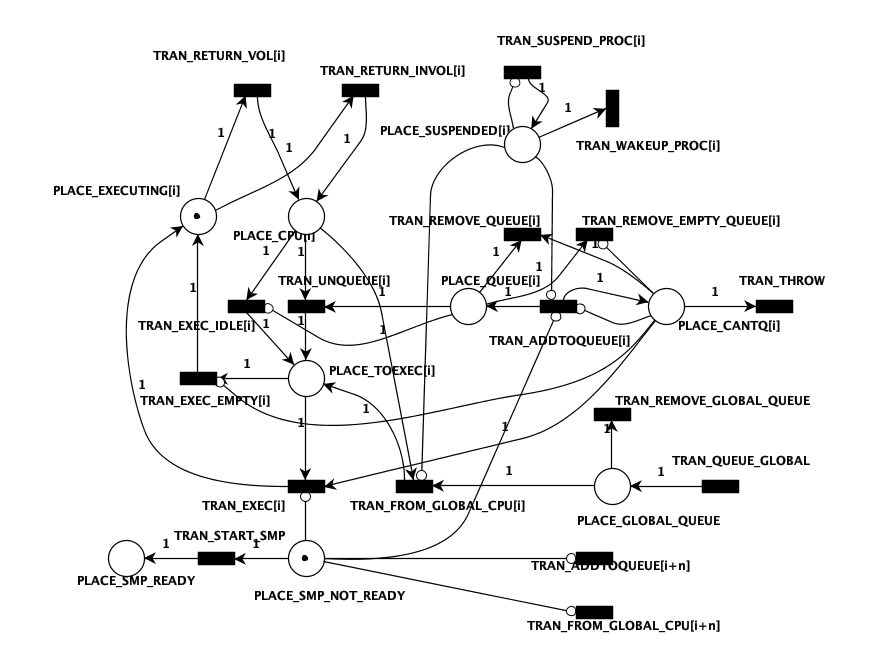
\includegraphics[width=0.8\textwidth]{./images/cpuOnOff-2nd-iteration.png}
    \caption{Segunda iteración del módulo de encendido/apagado de núcleos del procesador.}
    \label{fig:cpu-on-off-2nd-iteration}
\end{figure}

Una vez más, la implementación de estos cambios comenzó con la actualización de las matrices base y de incidencia. Después de realizar estos ajustes, se pudo proceder a incorporar las modificaciones correspondientes en el código del planificador. Dichos cambios incluyeron la implementación de la lógica detallada previamente, donde en casos de inactividad o inhabilitación manual de algún procesador, el flujo de ejecución de la red y, por tanto, de los procesos e hilos dentro de un núcleo, se comportará de manera esperada.\par

\begin{table}[H]
    \centering
    \begin{tabular}{|c|c|c|c|c|c|c|c|c|c|c|c|}
        \hline
        1 & 0  & -1 & 0  & \cellcolor{lightgray}0  & 0  & 0  & 0  & -1 & 0  & 0 & 0  \\
        \hline
        1 & -1 & 0  & 0  & \cellcolor{lightgray}0  & 0  & 0  & 0  & -1 & -1 & 0 & 0  \\
        \hline
        0 & -1 & 0  & 0  & \cellcolor{lightgray}-1 & 1  & 1  & -1 & 0  & 0  & 0 & 0  \\
        \hline
        0 & 1  & -1 & -1 & \cellcolor{lightgray}1  & 0  & 0  & 1  & 0  & 0  & 0 & 0  \\
        \hline
        0 & 0  & 1  & 1  & \cellcolor{lightgray}0  & -1 & -1 & 0  & 0  & 0  & 0 & 0  \\
        \hline
        0 & 0  & 0  & 0  & \cellcolor{lightgray}0  & 0  & 0  & 0  & 0  & 0  & 1 & -1 \\
        \hline
    \end{tabular}
    \caption{Matriz base: Segunda iteración del módulo de encendido/apagado.}
    \label{tabla:matriz_base_post_2}
\end{table}

\begin{table}[H]
    \centering
    \begin{tabular}{|c|c|c|c|c|c|c|c|c|c|c|c|}
        \hline
        1 & 0 & 0 & 1 & \cellcolor{lightgray}0 & 0 & 0 & 0 & 0 & 1 & 0 & 0 \\
        \hline
        0 & 0 & 0 & 0 & \cellcolor{lightgray}1 & 0 & 0 & 0 & 0 & 0 & 0 & 0 \\
        \hline
        0 & 0 & 0 & 0 & \cellcolor{lightgray}0 & 0 & 0 & 0 & 0 & 0 & 0 & 0 \\
        \hline
        0 & 0 & 0 & 0 & \cellcolor{lightgray}0 & 0 & 0 & 0 & 0 & 0 & 0 & 0 \\
        \hline
        0 & 0 & 0 & 0 & \cellcolor{lightgray}0 & 0 & 0 & 0 & 0 & 0 & 0 & 0 \\
        \hline
        1 & 0 & 0 & 0 & \cellcolor{lightgray}0 & 0 & 0 & 1 & 0 & 0 & 1 & 0 \\
        \hline
    \end{tabular}
    \caption{Matriz de incidencia: Segunda iteración del módulo de encendido/apagado.}
    \label{tabla:matriz_incidencia_post_2}
\end{table}

\subsection{Resultados}

Con la finalización del desarrollo de esta nueva funcionalidad, se procedió a realizar las pruebas correspondientes.\par

En resumen, la funcionalidad propuesta para el planificador, que permite habilitar o inhabilitar núcleos del procesador, ha sido implementada con éxito, proporcionando un control que antes no estaba disponible.\par

Además, se logró la versatilidad esperada para este módulo, ya que es posible activar esta mejora en ejecución sin necesidad de reiniciar el sistema operativo.\par

Los detalles completos de los resultados se discutirán en profundidad en el capítulo \ref{ch:results} de \textit{Análisis de Resultados}.\par

Es importante señalar que no es posible suspender el procesador cero. Esto se debe a que el sistema operativo utiliza este núcleo de forma predeterminada para tareas esenciales como la gestión de interrupciones, la gestión de memoria, entre otras; y al desactivarlo, el sistema experimenta un comportamiento inesperado. Para evitar esta situación, se realizaron ajustes en el código que impiden la selección de dicho núcleo para su suspensión.\par

\subsection{Próximos pasos}

La implementación de este módulo independiente no tiene un impacto inmediato en el sistema, ya que se activa únicamente cuando el usuario envía una señal específica, en el momento que elija.\par

De cara al futuro, creemos que el siguiente paso debería enfocarse en integrar esta funcionalidad con otros elementos clave del sistema operativo, como hilos, procesos o programas que los gestionen. Esta integración permitiría ajustar el estado de los procesadores en ejecución, respondiendo a las necesidades reales del sistema en su conjunto, y no solo a través de un módulo del kernel.\par

Otra mejora, relacionada con la estructura de la red de Petri de recursos desarrollada en la sección \ref{ch:idlethread}, sería asignar una plaza específica en la red para el \texttt{idlethread}. Esto facilitaría la detección de los momentos en los que el \texttt{idlethread} está en ejecución, proporcionando un mayor control sobre posibles acciones en estas situaciones.\par

\section{Módulo de monopolización de hilos por parte de los procesadores}

Tras finalizar el módulo de encendido y apagado de procesadores, nos enfocamos en el desarrollo del módulo de monopolización de hilos por parte de los procesadores. Este módulo introduce la capacidad en el planificador de anclar hilos a una CPU específica, lo que implica que dicho núcleo solo puede encolar y ejecutar los hilos que están asociados a él.\par

\subsection{Objetivos}

El objetivo de este módulo es proporcionar al planificador 4BSD la capacidad de anclar hilos a procesadores específicos en cualquier momento durante la ejecución del sistema operativo. Esto permitirá definir políticas de asignación de recursos más precisas y adaptables a las necesidades del sistema.\par

Es muy importante que este módulo, al igual que el desarrollado previamente, pueda ser cargado y activado en ejecución del sistema operativo, sin necesidad de reiniciarlo. Esta flexibilidad facilitará su integración con funcionalidades del sistema operativo, como la adaptación dinámica a cambios en la carga de trabajo o la asignación de hilos críticos a núcleos específicos para mejorar el rendimiento, entre otras.\par

\subsection{Primera Iteración: Desarrollo del Módulo de Monopolización a través de Políticas en la Red}

Para implementar el módulo de monopolización, se comenzó con una fase de investigación para explorar las posibles estrategias de desarrollo. Inicialmente, se consideró la opción de diseñarlo como un módulo independiente, similar al módulo de encendido/apagado. Sin embargo, se identificó que en última instancia, la decisión del planificador sobre a qué CPU encolar un hilo, estaba estrechamente vinculada a los identificadores de los hilos que se deseaban ejecutar.\par

Este enfoque nos llevó a entender el problema en términos de políticas para la toma de decisiones a la hora de encolar un hilo. Para implementar estas nuevas políticas, agregamos un mecanismo que permite fijar un hilo a un procesador específico, asegurándonos que dicho procesador no pueda encolar ni ejecutar otros hilos mientras esté monopolizado.\par

El proceso utiliza un nuevo registro (\verb|pinned_threads_per_cpu|) que rastrea el estado de monopolización de cada uno de los procesadores. Este registro se define como un arreglo de tantos elementos como procesadores en el sistema, que almacenan el identificador del hilo monopolizando dicho procesador (o -1 en caso de encontrarse libre). Así, cuando el planificador debe decidir donde ejecutar el hilo, primero verifica si este se encuentra \textit{anclado} a un procesador específico. Si es así, el hilo se encola en ese procesador para luego ser ejecutado. En caso contrario, el sistema sigue el proceso estándar de asignación a cualquier procesador disponible.\par

El comportamiento de la elección de procesador desarrollado, se muestra en la Figura \ref{fig:monopolization_resource-choose-cpu}.\par

\vspace{.50cm}
\begin{figure}[H]
    \centering
    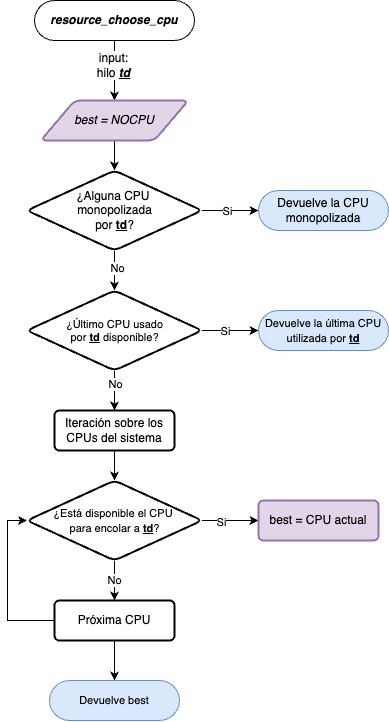
\includegraphics[width=0.35\textwidth]{images/monopolized_choose-cpu.png}
    \caption{Modelo de Monopolización de Hilos por Parte de los Procesadores.}
    \label{fig:monopolization_resource-choose-cpu}
\end{figure}

Junto con el desarrollo de este sistema, también desarrollamos funciones complementarias que permiten alternar el estado de monopolización de los procesadores, liberar un procesador cuando se decida, y verificar si un procesador está ocupado o disponible para un nuevo hilo.\par

Los detalles técnicos y las implementaciones específicas se encuentran documentados en el Apéndice \ref{appendix:apB}.\par

\subsection{Resultados}

Los resultados del módulo fueron satisfactorios, demostrando que los hilos pudieron monopolizar los procesadores de manera efectiva.\par

Para verificar este comportamiento, realizamos pruebas utilizando una herramienta de monitoreo y un programa de estrés. Estas pruebas consistieron en ejecutar diferentes programas diseñados para mantener hilos activos en los distintos núcleos de las CPUs durante un tiempo prolongado. Inicialmente, se observó el comportamiento global del sistema sin activar el módulo de monopolización. Luego, se seleccionó uno de estos hilos y se lo ancló a un procesador específico. Esto permitió comprobar que el módulo funcionaba correctamente, manteniendo los hilos anclados en un mismo núcleo sin que este pudiera ejecutar otras tareas, lo que confirma la efectividad de la monopolización.\par

Es importante señalar que el módulo no incluyó el caso de la CPU0, ya que, al igual que en pruebas anteriores con el módulo de encendido/apagado, presentaba dificultades para la monopolización debido a su rol en la gestión de tareas administrativas del sistema.\par

Los detalles específicos y un análisis más profundo de los resultados se abordarán en el capítulo de “Análisis de resultados”.\par

\subsection{Próximos pasos}

Aunque la implementación de este módulo no genera mejoras inmediatas en el sistema, su potencial radica en su activación bajo demanda, ya sea por señales específicas o por otras partes del kernel. Al igual que en el módulo anterior, su funcionalidad se activa solo cuando es necesario, lo que lo hace útil en escenarios concretos.\par

Este módulo puede ser particularmente beneficioso en situaciones donde se requiere garantizar la ejecución de tareas críticas en ejecución o cuando ciertos hilos necesitan acceso exclusivo y preferente a un procesador. Algunos ejemplos en los que podría ser beneficioso el módulo son en momentos de interrupciones de hardware a procesadores específicos, asegurando que estos hilos tengan acceso prioritario y minimizando la latencia en la respuesta a eventos de hardware. También podría ser útil en la gestión de dispositivos de almacenamiento de alto rendimiento, donde es crucial que los hilos responsables del acceso a disco mantengan un rendimiento constante.\par

Otra mejora significante del módulo, sería la de hacer que el mecanismo de anclaje sea más dinámico y flexible. Actualmente, el módulo permite anclar un solo hilo a un solo procesador, pero una posible extensión de esta funcionalidad podría permitir que un procesador ancle múltiples hilos simultáneamente. Esto permitiría una distribución más equilibrada de las cargas de trabajo.\par

Asimismo, se considera la posibilidad de que, en el futuro, se pueda anclar no solo hilos individuales, sino procesos enteros, asegurando que todos sus hilos se ejecuten exclusivamente en ese procesador.\par

\section{Tareas Extra}

Durante el proceso de desarrollo de los módulos, se fueron trabajando además algunas otras problemáticas encontradas.\par

\subsection{Modelado Específico de los Hilos \textit{Pinned}}

Durante el desarrollo de los módulos de encendido/apagado y monopolización de procesadores, surgió un problema crítico relacionado con la gestión de hilos \textit{pinned}, que ya había sido identificado en investigaciones anteriores.\par

En FreeBSD, los hilos \textit{pinned} deben ejecutarse exclusivamente en el procesador al que han sido asignados. En el contexto del planificador 4BSD modelado e implementado en la red de Petri de recursos, se modificó la lógica de selección de CPU. Originalmente, un hilo \textit{pinned} se reencolaba automáticamente en su procesador original sin condiciones adicionales. Sin embargo, con el desarrollo del modelo de la red de recursos, se introdujo una nueva condición: para que un hilo \textit{pinned} sea reencolado en su último procesador asignado, la transición que lo agrega a la cola del procesador debe estar habilitada.\par

Aunque esta modificación era necesaria para mantener el equilibrio en la carga de los núcleos del sistema, introdujo un problema adicional. Si, durante la ejecución de un hilo actual, se agrega otro hilo a la cola de ese procesador y simultáneamente se fija el hilo actual (es decir, se convierte en \textit{pinned}), la transición de reencolado del hilo \textit{pinned} podría quedar deshabilitada.\par

En tal situación, el planificador podría verse forzado a seleccionar un núcleo diferente o la cola global, lo que violaría la regla fundamental de los hilos \textit{pinned} del \textit{kernel} y podría provocar un \texttt{KERNEL PANIC}.\par

% \subsection{Solución del problema de afinidad (procesadores sobrecargados)}

% La primera de ellas, y la más crucial, fue un problema encontrado con la afinidad de los procesos.

% El síntoma ocurría durante nuestras pruebas de estrés; nos dimos cuenta de que los procesadores nunca alcanzaban el 100\% de su capacidad. Descubrimos que esto se debía a un problema de asignación de CPU que generaba una sobrecarga (overhead). El sistema operativo realizaba demasiados cambios de contexto entre los hilos, debido a un cambio en el código en relación con la afinidad, la limitación y la fijación a núcleos específicos.

% Estos cambios provocaban que el planificador eligiera los procesadores de forma aleatoria para encolar los hilos, sin considerar las indicaciones que podrían mejorar el rendimiento en la asignación de recursos y los cambios de contexto.

% % SKIPPED_TODO{IMAGEN DEL HTOP}

% A continuación, se dejan algunas pruebas de estrés realizadas previa y posteriormente a la implementación de la mejora. Si se observa detalladamente el programa htop en cada uno de los casos, se puede ver que en el primero, el promedio de uso de los procesadores es de un 78,62\% y el cálculo de todos los números primos hasta 100.000 tomó once segundos realizarlo (ocho veces, una por cada subproceso).

% En la segunda imagen, se muestran los resultados obtenidos al hacer los cambios correspondientes para mantener las funcionalidades de afinidad, limitación (bound) y la fijación a núcleos específicos (pin) en el planificador.

% Los cambios fueron positivos, logrando un uso pleno de los procesadores, que se mantuvieron al 100\% durante todas las pruebas de estrés realizadas y redujeron el tiempo de cálculo en un 63,63\%, completando la tarea en cuatro segundos.

% % SKIPPED_TODO{SEGUNDA IMAGEN DEL HTOP}


\subsection{Problema con la placa de red en el sistema operativo}\label{ch:problema_red}

Durante el desarrollo del proyecto integrador, identificamos un problema recurrente relacionado con el uso de la placa de red en nuestra máquina virtual. Este inconveniente surgía específicamente al utilizar SSH para facilitar la conexión con la máquina. Sin embargo, cuando se desactivaba la placa de red antes de iniciar la máquina virtual, el problema no ocurría, aunque esto también impedía el uso de SSH.\par

El problema técnico consistía en un \textit{kernel} panic provocado por un page fault durante el arranque del sistema operativo. Luego de cada incidente, el sistema generaba un archivo con información del estado previo al fallo, lo que nos permitió realizar un análisis más detallado.\par

Para abordar la situación, recurrimos al foro oficial de FreeBSD, donde presentamos nuestro caso. La discusión nos brindó diversas perspectivas y posibles soluciones, pero no logramos resolver el problema. Este intercambio de ideas se encuentra documentado en el hilo titulado \emph{"Kernel panics when given a high workload, accesible en el foro oficial de FreeBSD"}\cite{bib6}.\par

Aunque no encontramos una solución definitiva, este proceso nos permitió adquirir conocimientos valiosos. Aprendimos a utilizar herramientas avanzadas para depurar el kernel, a interpretar archivos de crash dump generados durante los fallos y confirmamos que la comunidad de FreeBSD tiene un fuerte interés en iniciativas relacionadas con planificadores basados en Redes de Petri. Además, demostraron una disposición notable para ayudar en casos similares.\par

Consideramos que este es un punto relevante para futuras investigaciones y mejoras. Si bien no se trata de un problema bloqueante, su solución podría contribuir significativamente a mejorar la experiencia de desarrollo y operación del sistema.\par

Las capturas de pantalla y el análisis detallado del fallo se encuentran documentados en el Apéndice \ref{appendix:apC}.\par